\documentclass[tikz]{standalone}

\pagestyle{empty}

\usepackage{amsmath}
\usepackage{tikz}
\usepackage{graphicx}
\usetikzlibrary{positioning,calc,fit,decorations.pathreplacing,arrows,positioning,backgrounds}

% Font settings:
\renewcommand{\familydefault}{\sfdefault}
\usepackage{pxfonts}
\newcommand{\figf}{\sffamily\bfseries\small} %Defines the font used for the labelling of figure panels.


% Color settings:
%\definecolor{hivc}{cmyk}{0,0.80,0.83,0.13}                %\definecolor{hivc}{HTML}{DE2D26}
\definecolor{hivc}{RGB}{24,116,205}
\definecolor{selfc}{cmyk}{0,0,0,0.6}                      %\colorlet{selfc}{gray!80!white}
\definecolor{Rblue}{RGB}{100,149,237}



%__________________________________________________________________________
%__________________________________________________________________________
%%----BEGINNING OF DOCUMENT
%__________________________________________________________________________
%__________________________________________________________________________

\begin{document}
\scriptsize

%---------------------------------FIGURE 1: LANGUAGES---------------------------------

\begin{tikzpicture}[anchor=north west]
%\filldraw[white] (0,0) rectangle (17.92445,-0.1);
%\filldraw[white] (0,0) rectangle (12,-0.1);
\clip (0,0) rectangle (12,-9.5);


% PANEL A
\begin{scope}[]
  \node[anchor = north west] at (0.2,0) {\includegraphics{../cartoons/plots/contiguous_lang2.pdf}};
  \node at (0,0) {\figf  A};
\end{scope}

% PANEL B
\begin{scope}[yshift=-2.cm]
  \node[scale=1, anchor = north west] at (0,0) {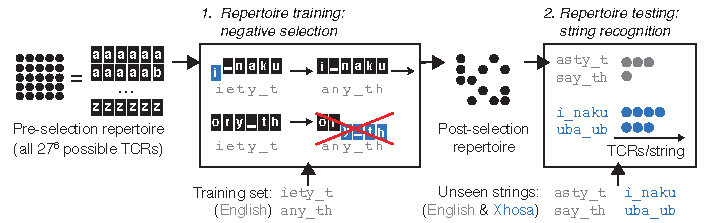
\includegraphics{../cartoons/plots/negative-selection.pdf}};
  \node at (0,0) {\figf  B};
\end{scope}

% PANEL C
\begin{scope}[yshift=-5.9cm]
  \node[anchor = north west, scale=0.75] at (1.85,-0.5) {\includegraphics{../../figure-languages/plots/Xhosa-example-r3-n500.pdf}};
  \node[anchor = north west, scale=0.75] at (0,-0.5) {\includegraphics{../../figure-languages/plots/Xhosa-example-r3-n0.pdf}};
  \node at (1.1,-0.35) {Before selection:};
  \node at (3.05,-0.35) {After selection:};
  \node at (0,-0.1) {\figf  C};
\end{scope}

% PANEL D
\begin{scope}[xshift=4.9cm, yshift=-5.9cm]
  \node[anchor = north west, scale=0.75] at (0,-0.35) {\includegraphics{../../figure-languages/plots/pf-xh-r3.pdf}};
  \node[hivc, anchor = east, align=left] at (3.25,-0.55) {Xhosa};
  \node[selfc, anchor = east, align=left] at (3.25,-2.0) {English};
  \node at (0,-0.1) {\figf  D};
\end{scope}

% PANEL E
\begin{scope}[xshift=8.3cm, yshift=-5.9cm]
  \node[anchor = north west, scale=0.75] at (0,-0.5) {\includegraphics{../../figure-languages/plots/top-xh-r3.pdf}};
  \node at (0,-0.1) {\figf  E};
\end{scope}


\end{tikzpicture}

\end{document}